% Chapter 4

\chapter{Experiment} % Write in your own chapter title
\label{Chapter4}
\lhead{Chapter 4. \emph{Experiment}}

The experiment environment includes hardware, which is i7 CPU, 8G RAM and a GeForce GTX 770, and software, which is Ubuntu Linux 14.04 and Caffe \citep{jia2014caffe}, a deep learning software framework.

\section{Training Neural Networks}

We trained the model with the 1000-category ImageNet2012 dataset. We used the network architecture ~\cite{ZeilerF13} which achieved an excellent accuracy in the 2013 ImageNet Competition. We implemented SPP with CUDA C language and deployed it before the first fully connected layer.

In the experiment, a subset of the ImageNet dataset, which contains 1.2 million labelled high-resolution images depicting 1,000 object categories and 50,000 validation images, was used as training dataset. Most images are multi-scale and some are grey. To feed them into the network conveniently, the images were converted to the same dimensions , $256\times256$. Grey images were combined triple times to simulate RGB images. The model was trained on raw RGB values of pixels. The activation function is the ReLU, which guarantees fast training of the neural network.

\begin{equation}\label{eq:ReLU}
f(x) = max(0, x)
\end{equation}

The model \ref{fig:ImageNetArch} was trained with a descent optimisation method, SGD. The batch size is 128, and the momentum is 0.9.  In each layer, the weights are initialised with a Gaussian distribution which has the mean of $0$, and the standard deviation of $0.01$. The neuron bias, in the $Conv_{2}$, $Conv_{4}$, $Conv_{5}$ and fully connected layers, was initialised with value 1, while the other bias was initialised with value 0.

The learning rates are set equally for all layers. They are initialised at 0.01 and decrease with the stepdown policy which means that they would drop by a factor of 10 after each 100,000 iterations. In total, the learning rates drop 3 times and the accuracy keeps stable after 370,000 iterations. 

The training is regularised via the techniques, including dropout and weight decay. The dropout regularisation is implemented at the two fully connected layers and the dropout ratio is 0.5. The neurons, which are dropped out, output zero and do not participate in the backpropagation process. Therefore, the neural network samples different architectures each time. This significantly decreases complex co-adaptations of neurons because they do not depend on the existence of other neurons. The weight decay, $\epsilon$, is set to 0.0005 which means the new weights are shrunk according to 
\begin{equation}\label{eq:WeightDecay}
w^{new} = w^{old}(1 - \epsilon)
\end{equation}
after each updating.

\section{Fine-tuning Model}

There are two challenges to training on the original model. Firstly, the original CNN model is trained to classify images of $1,000$ categories. However, the current task is to classify two weather scenes. This can be solved by reducing the outputs of the last fully connected layer from $1,000$ to $2$. Secondly, the CNN architecture contains about $60$ million parameters which are too many for the weather classification dataset. The target dataset has only $10,000$ images in total. The number of images is insufficient and the model is feasible to overfit. It can be solved by training a new model based on the pre-trained CNN model. Because the pre-trained model is close to optimism, it only needs a tiny adjustment.

The fine-tune transfers the weights of each layer from the pre-trained model to the new model except for the last fully connected layer. The last layer is taken over by a new layer which contains the same amount of neurons equally to the class number. The weights in the replaced layer are initialised with random values. One advantage of fine-tune is to minimise risk of overfitting. The other one is that weights reach optimal values quickly.

$9,000$ images are used for training and $1,000$ images are reserved to test the model. The batch size is $128$. There are $10,000$ iterations in the training process totally. Then the total training image number is $128\times9,000$. One epoch is that the total training images are fed into the network once. The training epochs are $142$. The initial base learning rate is $0.001$ and the rate is divided by $10$ every $10$ epochs. Because the weights in $FC8$ are randomly initialised and they are not close to final optimisation value, the learning rate for $FC8$ is $10$ times of the base learning rate to converge quickly.

\section{Companion Experiments}

In order to compare performance of the fine-tuned model, we did extra tests with extracting feature methods. We used a pre-trained model with the AlexNet architecture and extracted features from the layer $FC7$. We trained a SVM classifier based on the features and classified the test samples.

\section{Experimental Results}

The results in Table \ref{ExpRes} illustrate that the models, trained by the neural networks, have better performance than the extracting features method. 

\begin{table}[h]
\begin{center}
    \begin{tabular}{| c | c | c | c | c |}
    \hline
    Methods & CNN+SVM & SPP+SVM & Finetune on CNN & Finetune on SPP  \\ \hline
    Accuracy & $84.8\%$ & $82.1\%$ & $93.1\%$ & $93.98\%$ \\ \hline
    \end{tabular}
    \caption{The first test is extracting features from the pre-trained CNN model and training a SVM classifer. The second test is similar with the first except for extracting features from the CNN model with a SPP layer. The third test is fine-tuning the model with AlexNet architecture. The fourth test is fine-tuning the CNN model with a SPP layer}
    \label{ExpRes}
\end{center}
\end{table}

The fine-tuning process converges quick. After about 30 epochs, the accuracy rate exceeds $90\%$. 
\graphicspath{ {./Figures/} }
\begin{figure}[!htb]
    \centering
	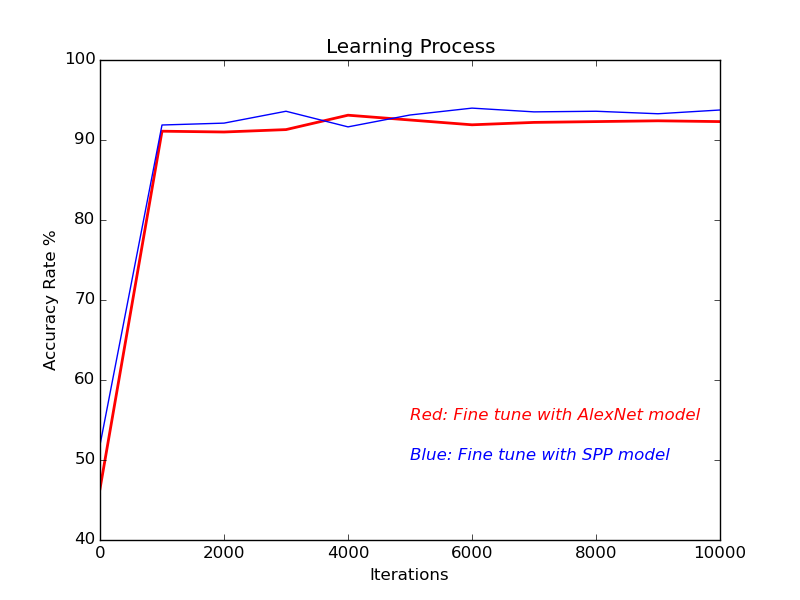
\includegraphics[width=0.8\textwidth]{FinetuneAccuracy.png}
    \caption{Learning Process}%
    \label{fig:finetuneprocess}%
\end{figure}

The learning process may overfit and it will definitely damage model generalisation capability. From Figure \ref{fig:finetuneprocess}, it shows that there is no overfitting in the fine-tuning process.

In order to have a more detailed information of the fine-tuning process, we investigate the training loss values. We plot the curve and the loss values during the first 200 iterations.

\begin{figure}[!htb]
    \centering
	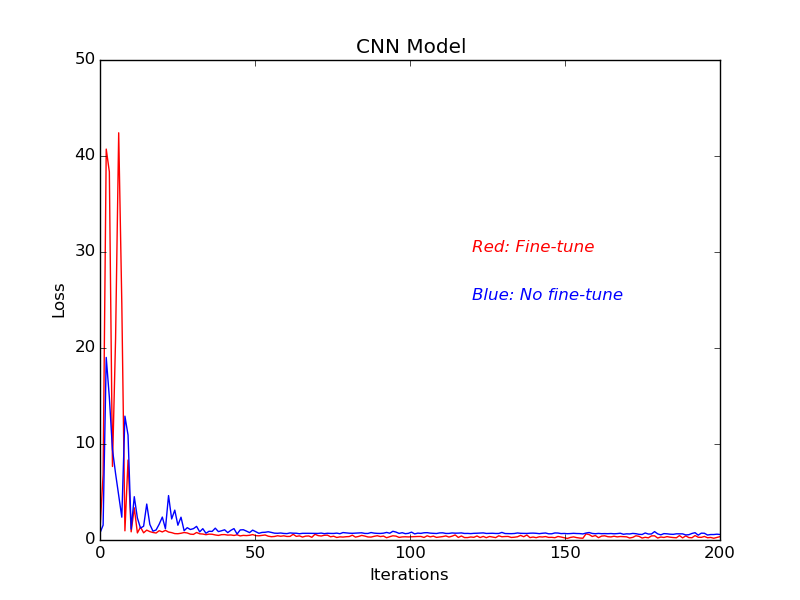
\includegraphics[width=0.4\textwidth]{finetuneCNNProcess.png}
	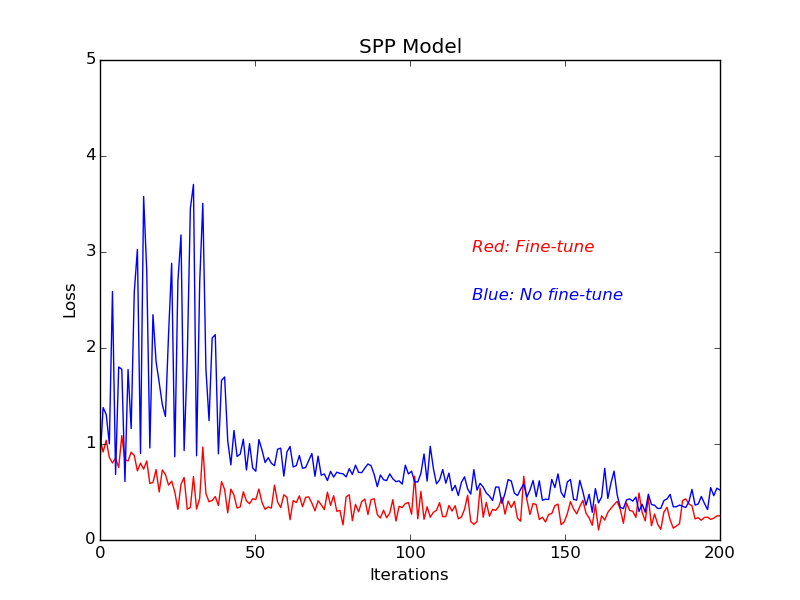
\includegraphics[width=0.4\textwidth]{finetuneSPPProcess.png}
    \caption{Training Loss}%
    \label{fig:FTvsSC}%
\end{figure}

From Figure \ref{fig:FTvsSC}, it is clear that the fine-tuning process produces a smoother loss curve and ceases at a higher accuracy rate. In the left figure, the loss value of the fine-tuning procedure is higher than the value of the non fine-tuning process at the beginning. Then it shrinks sharply and maintains lower than the value of the non fine-tuning process. In the right figure, we can find that the initial loss value is less than that in the left figure. And the loss value of the fine-tuning process is less than the value in the non fine-tuning process. In summery, fine-tuning is an effective approach to training a new model. The model with SPP layers achieved high performance.

\begin{figure}[!htb]
    \centering
	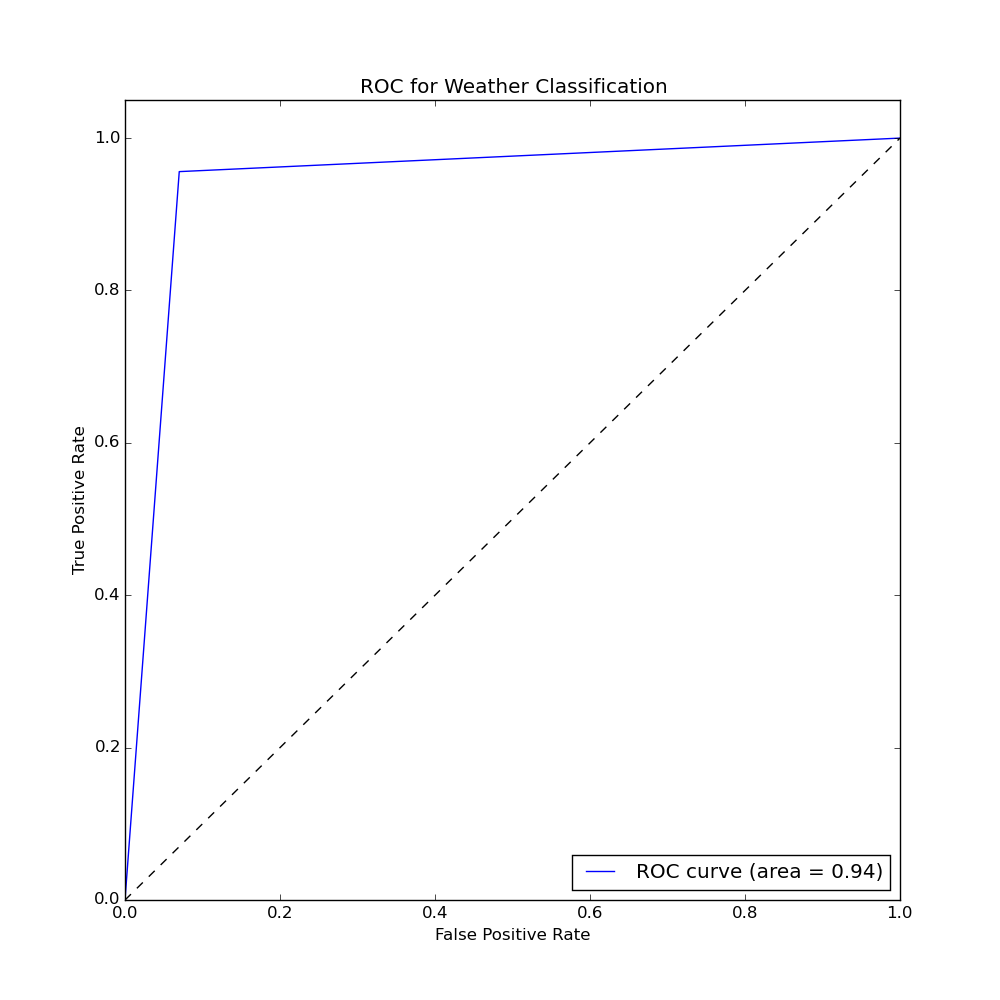
\includegraphics[width=0.8\textwidth]{ROCWeatherClassification.png}
    \caption{ROC Curve}%
    \label{fig:WeatherClassificationROC}%
\end{figure}

\section{Architecture Analysis}

CNN has achieved excellent accuracy in object classification, although a full understanding of the mechanism is ambiguous. In order to have some intuition about CNN, we will analyse the network outputs.

The outputs of each convolutional layer have been treated as visual descriptors \citep{razavian2014cnn}, and the vectors present some information from the outputs of previous layers. The front layers encode low-level features, and the rear layers are able to capture high-level features. In summary, an image is retrieved heuristically when it passes the convolutional layers.

Fully connected layers can be represented as a $d$-dimensional vector. The layer takes multidimensional outputs from the previous layer and flats the feature maps into a $d$-dimensional vector. The outputs of the second fully connected layer are fed into a classifier.

When a cloudy image is fed into the CNN, Figure \ref{fig:cloudy_finetuneprocess} shows the feature maps of convolutional layers. Because the filter size is too many, only parts of the filters are plotted in b-f.

\graphicspath{ {./Figures/DifferentLayers/} }

\begin{figure}[htb]
    \centering
    \subfigure[raw image]{
		\begin{minipage}{0.3\textwidth}
		   		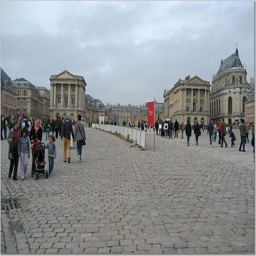
\includegraphics[width=1\textwidth]{cloudy1}
		   		\label{fig:cloudy}
		\end{minipage}
    	} 
    \subfigure[conv1 output]{
		\begin{minipage}{0.3\textwidth}
		   		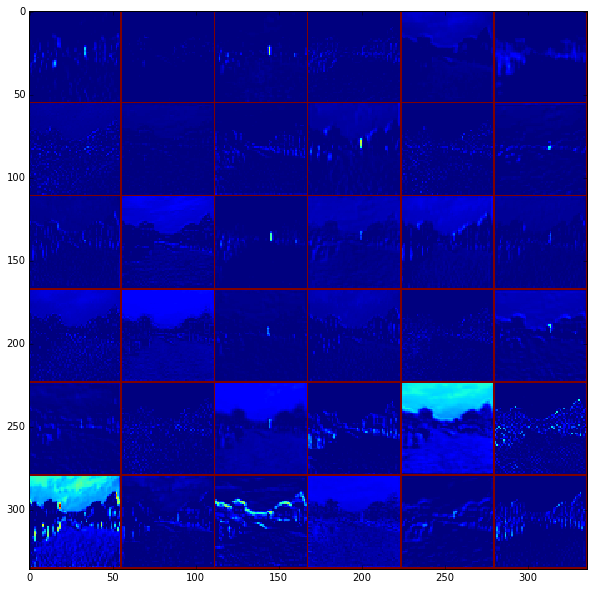
\includegraphics[width=1\textwidth]{cloudy1_conv1_fm}
		   		\label{fig:cloudy_conv1}
		\end{minipage}
    	} 
    \subfigure[conv2 output]{
		\begin{minipage}{0.3\textwidth}
		   		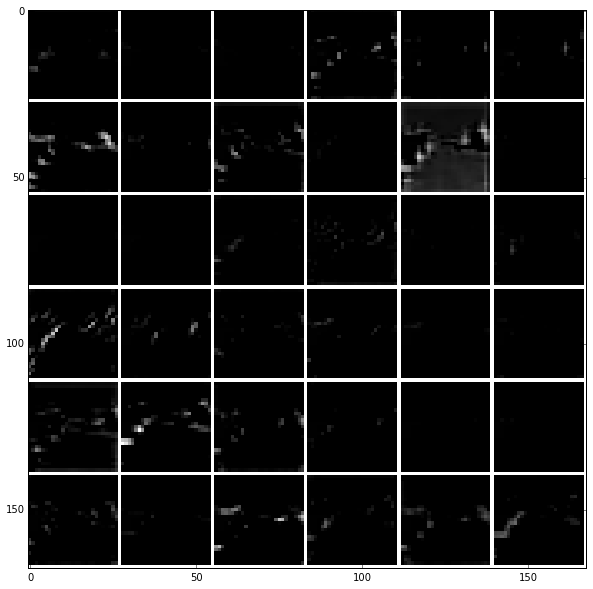
\includegraphics[width=1\textwidth]{cloudy1_conv2_fm}
		   		\label{fig:cloudy_conv2}
		\end{minipage}
    	} 
    \subfigure[conv3 output]{
		\begin{minipage}{0.3\textwidth}
		   		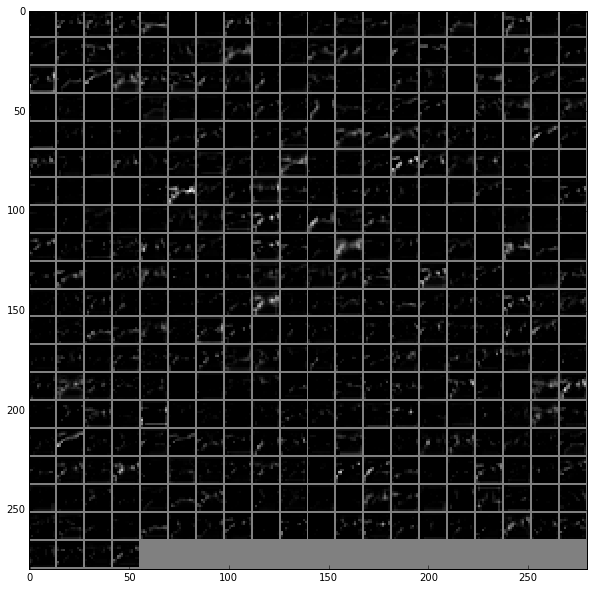
\includegraphics[width=1\textwidth]{cloudy1_conv3_fm}
		   		\label{fig:cloudy_conv3}
		\end{minipage}
    	} 
    \subfigure[conv4 output]{
		\begin{minipage}{0.3\textwidth}
		   		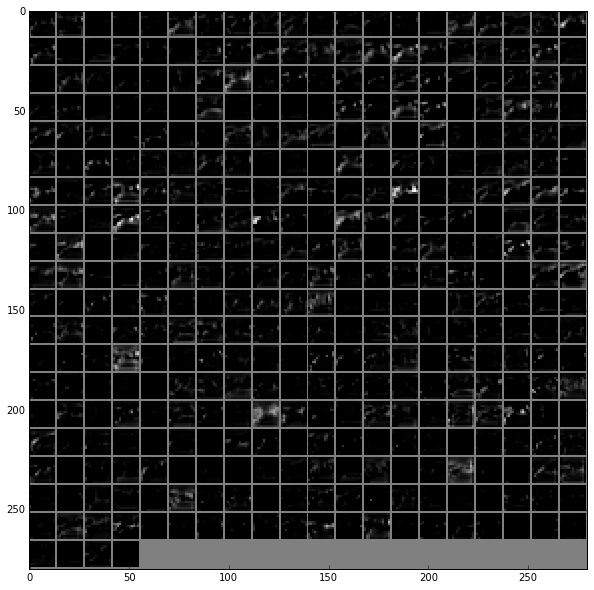
\includegraphics[width=1\textwidth]{cloudy1_conv4_fm}
		   		\label{fig:cloudy_conv4}
		\end{minipage}
    	} 
    \subfigure[conv5 output]{
		\begin{minipage}{0.3\textwidth}
		   		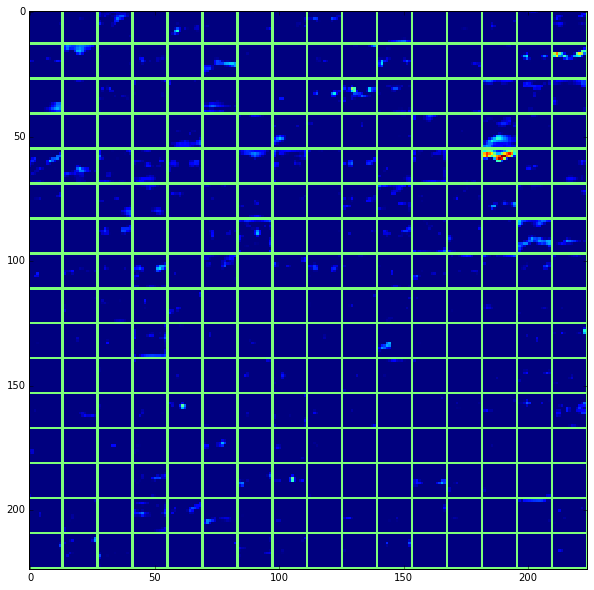
\includegraphics[width=1\textwidth]{cloudy1_conv5_fm}
		   		\label{fig:cloudy_conv5}
		\end{minipage}
    	} 

    \caption{A cloudy image and the feature maps from convolutional layers}%

    \label{fig:cloudy_finetuneprocess}%
\end{figure}

In Figure \ref{fig:sunny_finetuneprocess}, a sunny image is fed into the CNN and the according outputs are plotted.

\begin{figure}[!htb]
    \centering
    \subfigure[raw image]{
		\begin{minipage}{0.3\textwidth}
		   		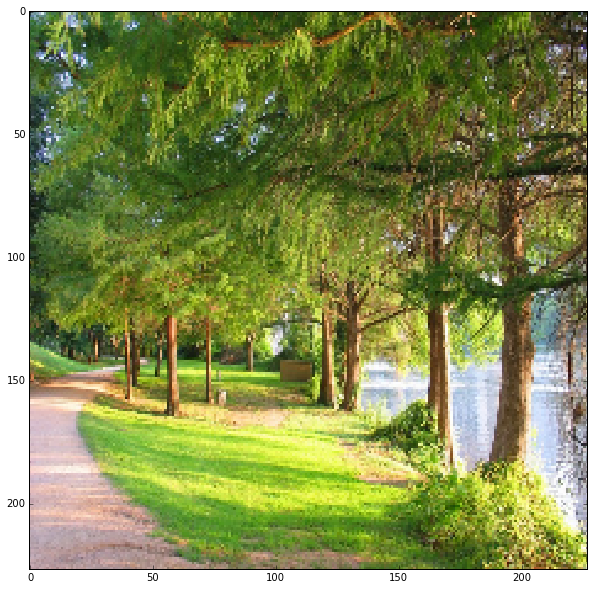
\includegraphics[width=1\textwidth]{sunny2}
		   		\label{fig:sunny_ft}
		\end{minipage}
    	} 
    \subfigure[conv1 output]{
		\begin{minipage}{0.3\textwidth}
		   		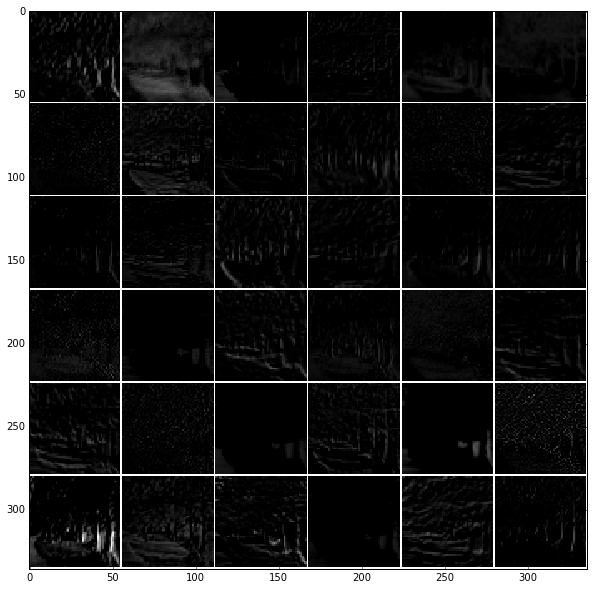
\includegraphics[width=1\textwidth]{sunny2_conv1_fm}
		   		\label{fig:sunny_ft_conv1}
		\end{minipage}
    	} 
    \subfigure[conv2 output]{
		\begin{minipage}{0.3\textwidth}
		   		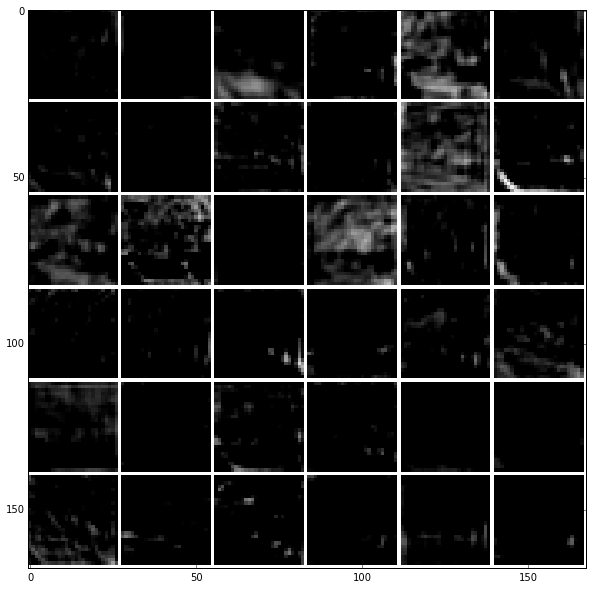
\includegraphics[width=1\textwidth]{sunny2_conv2_fm}
		   		\label{fig:sunny_ft_conv2}
		\end{minipage}
    	} 
    \subfigure[conv3 output]{
		\begin{minipage}{0.3\textwidth}
		   		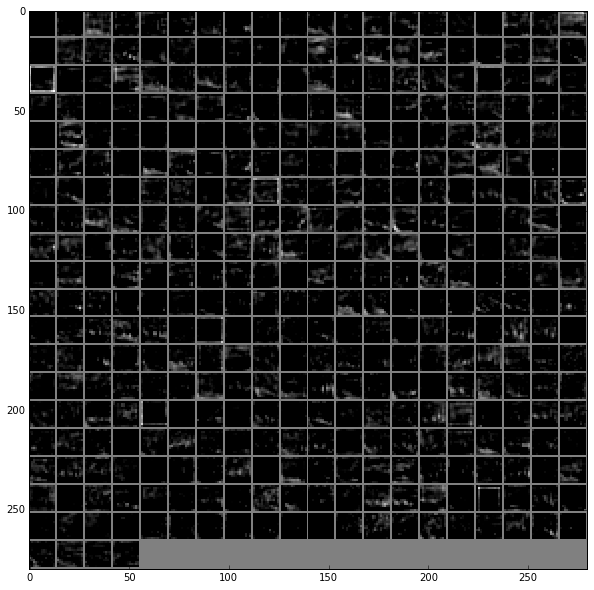
\includegraphics[width=1\textwidth]{sunny2_conv3_fm}
		   		\label{fig:sunny_ft_conv3}
		\end{minipage}
    	} 
    \subfigure[conv4 output]{
		\begin{minipage}{0.3\textwidth}
		   		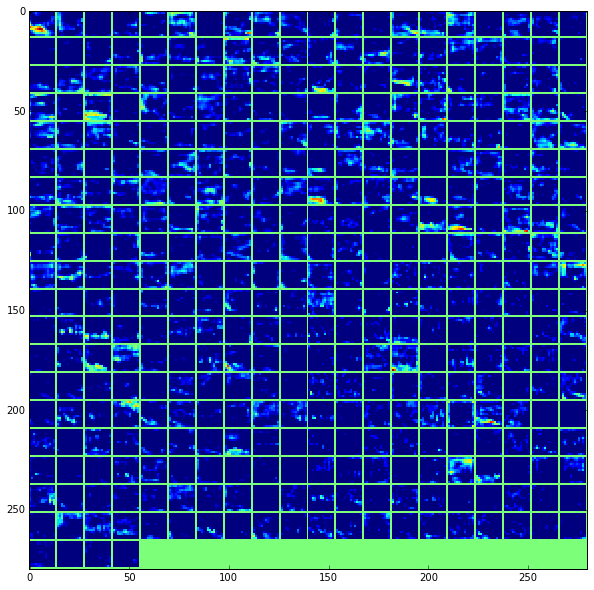
\includegraphics[width=1\textwidth]{sunny2_conv4_fm}
		   		\label{fig:sunny_ft_conv4}
		\end{minipage}
    	} 
    \subfigure[conv5 output]{
		\begin{minipage}{0.3\textwidth}
		   		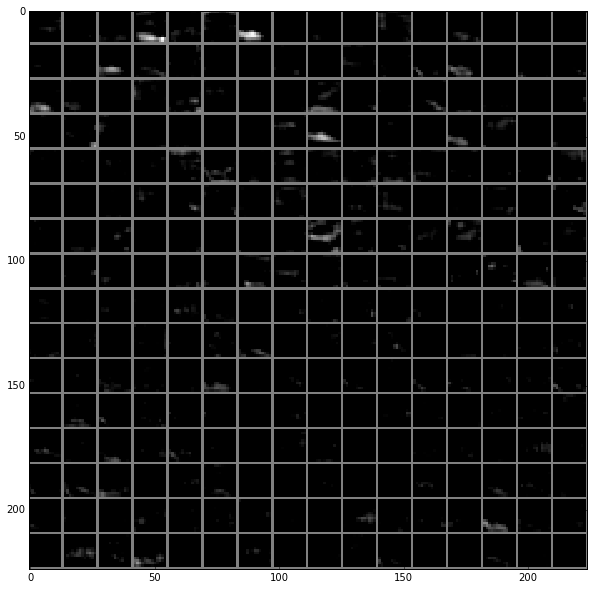
\includegraphics[width=1\textwidth]{sunny2_conv5_fm}
		   		\label{fig:sunny_ft_conv5}
		\end{minipage}
    	} 

    \caption{A sunny image and the feature maps from convolutional layers}%

    \label{fig:sunny_finetuneprocess}%
\end{figure}

The outputs of $CONV1$ and $CONV2$ are still partly recognisable by people. The outputs of $CONV3$ and $CONV4$ are unrecognisable. From the outputs of $CONV5$ for the sunny image, the position of sun light is highlighted by several filters. However, the according filters show no signs about the cloudy image.

\section{Effects of SPP Layer}

The outputs of SPP layers cannot be represented as visual descriptors, then only the feature maps of the convolutional layers are compared in the models. The outputs of $CONV1$ and $CONV2$ show that more features are recognisable in the SPP model. It illustrates that the SPP model has stronger representation capability than the CNN model does.
 
\begin{figure*}[!htb]
\begin{center}

\begin{tabular}{|c|c|c|c|c|c|} \hline\hline
Image & Conv1 & Conv2 & Conv3 & Conv4 & Conv5  \\ \hline
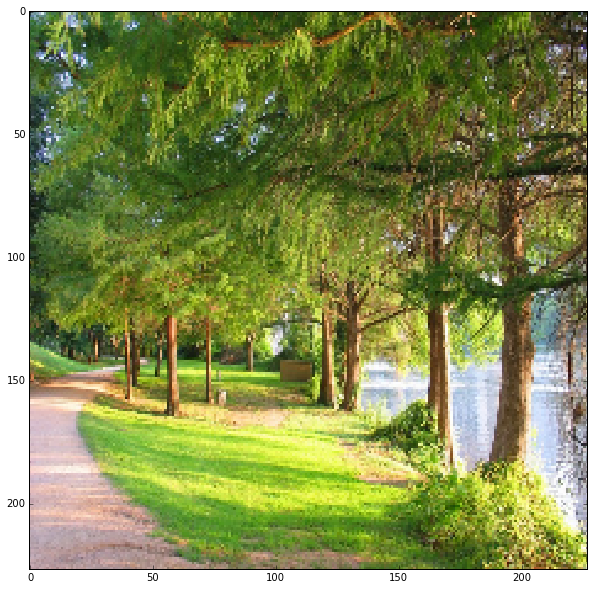
\includegraphics[scale=0.1]{sunny2.png} &
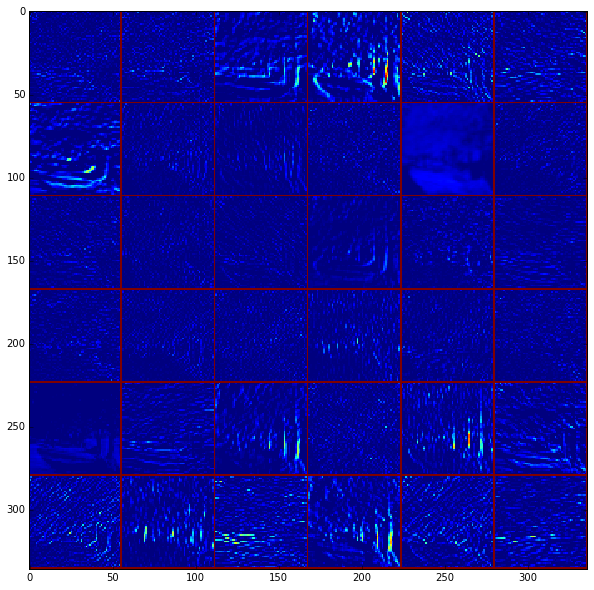
\includegraphics[scale=0.1]{sunny2_caffe_conv1_fm.png} &
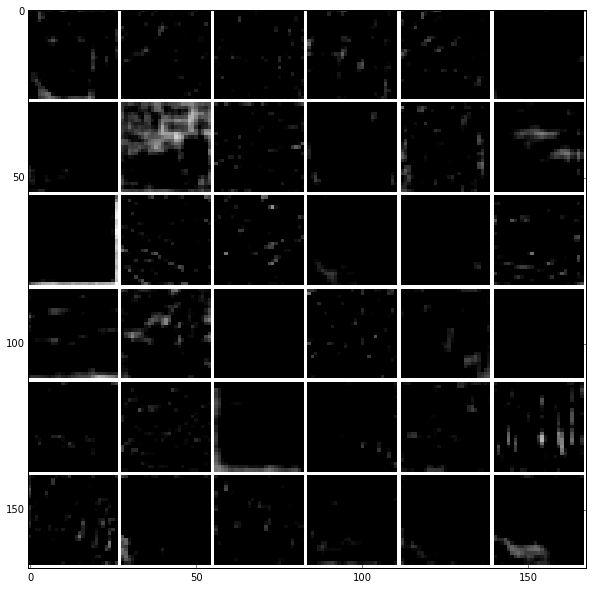
\includegraphics[scale=0.1]{sunny2_caffe_conv2_fm.png} &
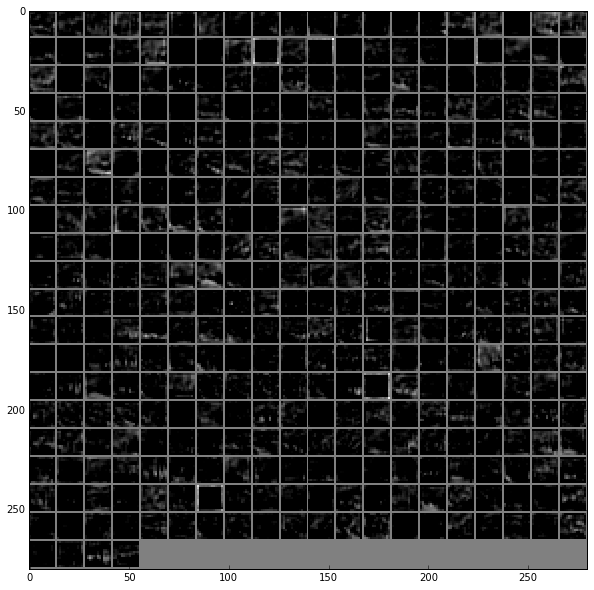
\includegraphics[scale=0.1]{sunny2_caffe_conv3_fm.png} &
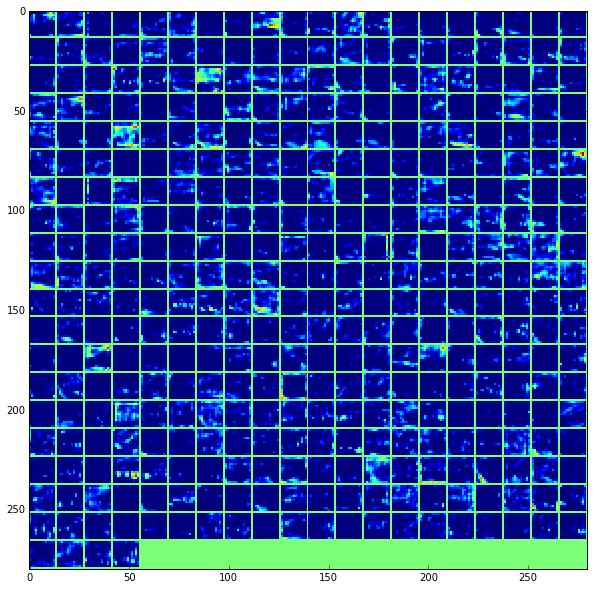
\includegraphics[scale=0.1]{sunny2_caffe_conv4_fm.png} &
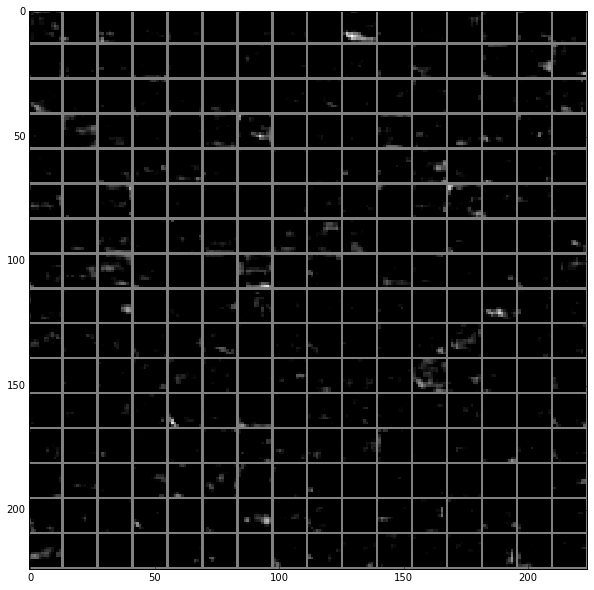
\includegraphics[scale=0.1]{sunny2_caffe_conv5_fm.png}\\ \hline\hline

Image & Conv1 & Conv2 & Conv3 & Conv4 & Conv5  \\ \hline
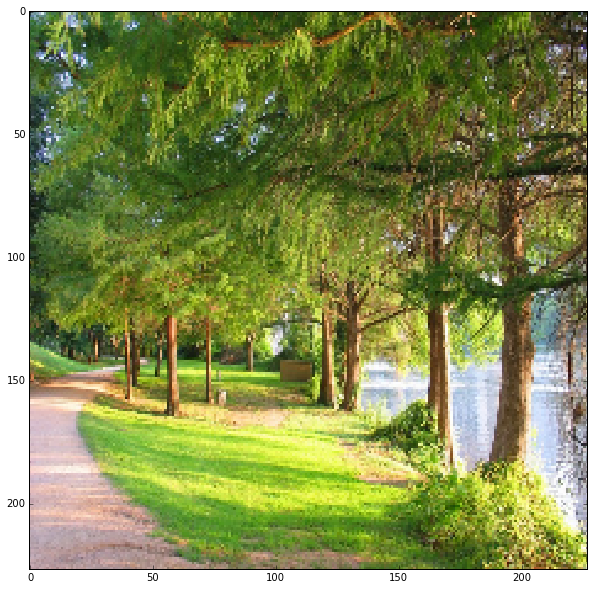
\includegraphics[scale=0.1]{sunny2.png} &
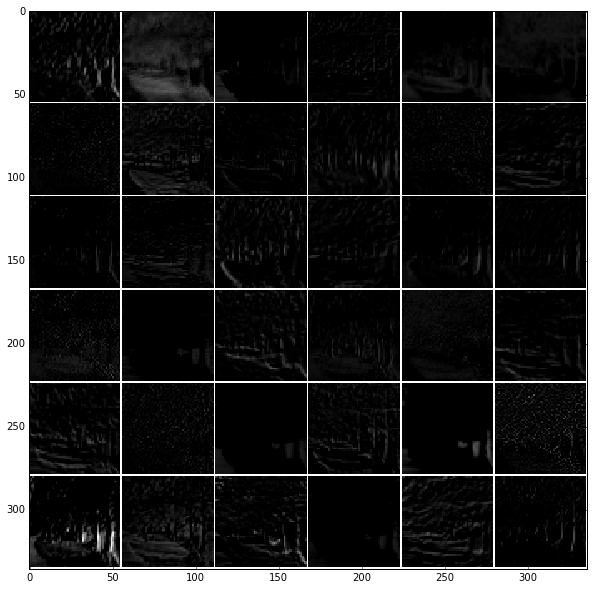
\includegraphics[scale=0.1]{sunny2_conv1_fm.png} &
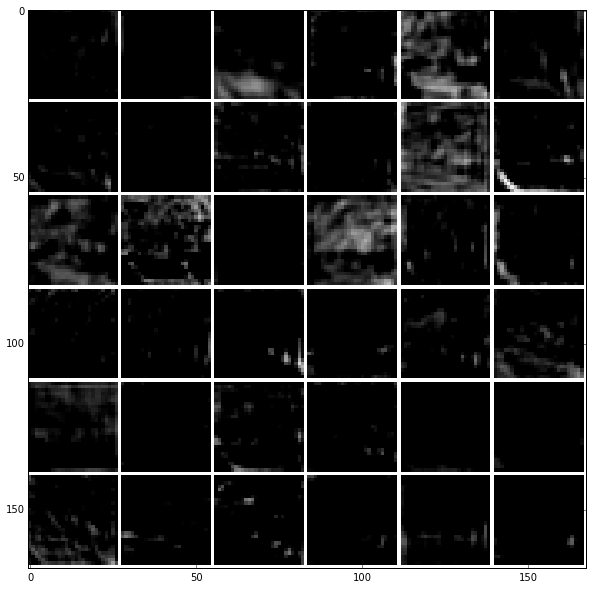
\includegraphics[scale=0.1]{sunny2_conv2_fm.png} &
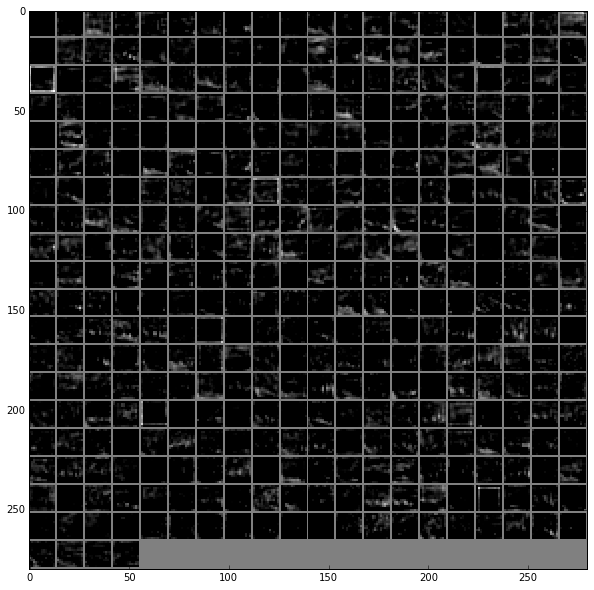
\includegraphics[scale=0.1]{sunny2_conv3_fm.png} &
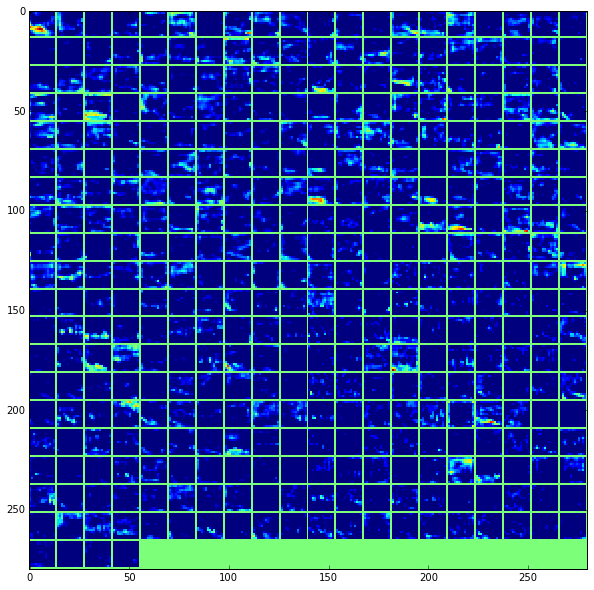
\includegraphics[scale=0.1]{sunny2_conv4_fm.png} &
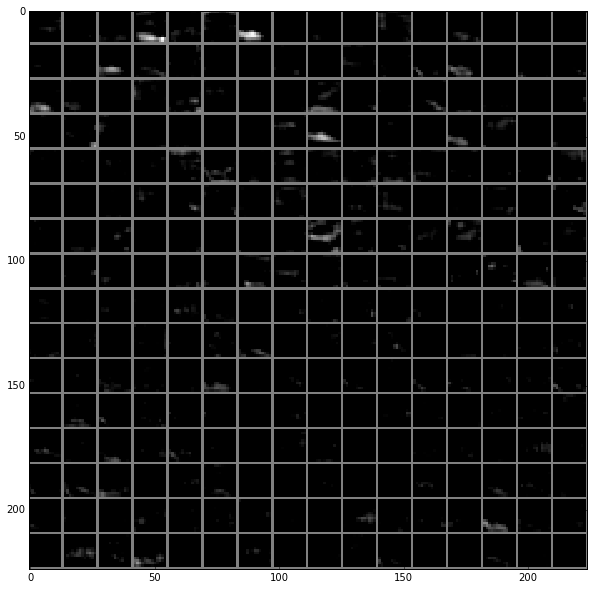
\includegraphics[scale=0.1]{sunny2_conv5_fm.png}\\ \hline\hline
\end{tabular}

\end{center}
	\caption{Visiualisation of feature maps from the CNN model and the SPP model. The upper images are from the CNN model and the lower images are from the fine-tuned model.}
	\label{fig:diff_featuremap}%
\end{figure*}

In Figure \ref{fig:fc7_hist_output}, the histograms of the outputs from the layer $FC7$ are displayed. Comparing histogram difference, the generated features of the SPP model is more divisible than those of the CNN model.
\begin{figure}[htb]
    \centering
	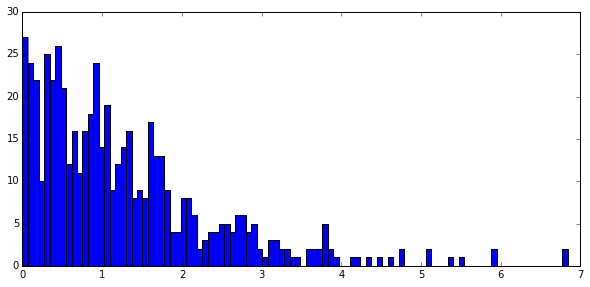
\includegraphics[width=0.4\textwidth]{sunny2_hist_caffe_fc7.png}
	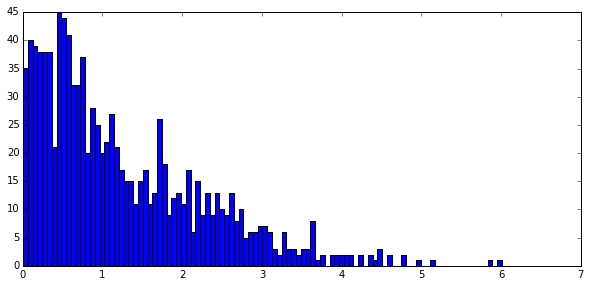
\includegraphics[width=0.4\textwidth]{sunny2_hist_spp_fc7.png}
    \caption{Histogram distribution of vectors from FC7. The left is from CNN model and the right is from the SPP model.}%
    \label{fig:fc7_hist_output}%
\end{figure}

From the feature maps and histogram distributions, it is clear that the SPP model has strong representing capability and can generate divisible features to classifiers.

\section{Error Results}

The images in Figure \ref{fig:Misclassification} are misclassified by the CNN model and the SPP Model. They are difficult to judge sunny or cloudy, even for people.
\graphicspath{ {./Figures/} }
\begin{figure}[htb]
    \centering
    \subfigure[sunny]{
		\begin{minipage}{0.3\textwidth}
		   		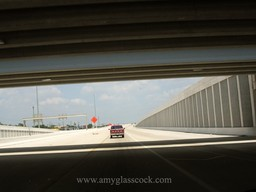
\includegraphics[width=1\textwidth]{err_sunny1}
		   		\label{fig:sunny}
		\end{minipage}
    	} 
    \subfigure[sunny]{
		\begin{minipage}{0.3\textwidth}
		   		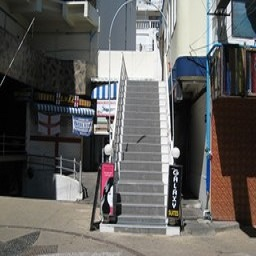
\includegraphics[width=1\textwidth]{err_sunny2}
		   		\label{fig:sunny_conv1}
		\end{minipage}
    	} 
    \subfigure[sunny]{
		\begin{minipage}{0.3\textwidth}
		   		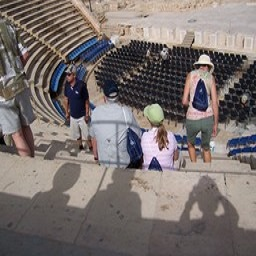
\includegraphics[width=1\textwidth]{err_sunny3}
		   		\label{fig:sunny_conv2}
		\end{minipage}
    	} 
    \subfigure[cloudy]{
		\begin{minipage}{0.3\textwidth}
		   		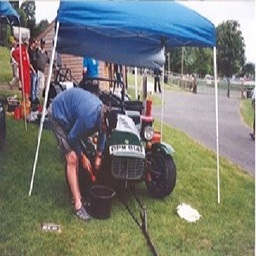
\includegraphics[width=1\textwidth]{err_cloudy1}
		   		\label{fig:sunny_conv3}
		\end{minipage}
    	} 
    \subfigure[cloudy]{
		\begin{minipage}{0.3\textwidth}
		   		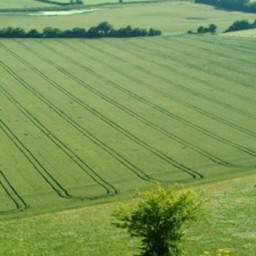
\includegraphics[width=1\textwidth]{err_cloudy2}
		   		\label{fig:sunny_conv4}
		\end{minipage}
    	} 
    \subfigure[cloudy]{
		\begin{minipage}{0.3\textwidth}
		   		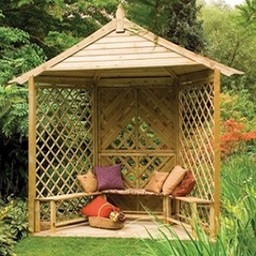
\includegraphics[width=1\textwidth]{err_cloudy3}
		   		\label{fig:sunny_conv5}
		\end{minipage}
    	} 
    \caption{Misclassified images \citep{lutwo}.}%
    \label{fig:Misclassification}%
\end{figure}

\section{Conclusion and Future Work}

In this experiment, we present an effective approach to perform weather classification through CNN and transfer learning. The results illustrate the strong capacity of CNN and the convenience of transfer learning. Compared with the shallow learning methods, which extract features and train a classifier, the CNN method does not depend on specific feature detectors and achieves high accuracy. 

In the future, the full understanding of the CNN mechanism is a demanding work. And the work can be extended to multi-class weather classification and will be implemented in industry widely.